\documentclass{report}
\usepackage{longtable}
\usepackage{listings}
\usepackage{graphicx}
\usepackage{multirow}
\usepackage{fontspec}
\usepackage[section]{placeins}

\newfontfamily{\ttconsolas}{Consolas}

\title{Lab6\_Ripple Carry Adder design}
\author{201704150 Kangjun Heo}

\lstset{basicstyle=\ttfamily,breaklines=true}
\lstset{framextopmargin=10pt,framexbottommargin=10pt,frame=tb}


\begin{document}
    \maketitle
    \tableofcontents

    \chapter{Purpose of the lab}

        \paragraph{This lab aims to design 8-bit Ripple Carry Adder with Verilog language. This report contains Truth table, Boolean equation, Karnaugh map and Logic diagram.}
    
        \section{Ripple Carry Adder}

        \paragraph{\normalfont Ripple Carry Adder is a adder that consists of Full Adders, that outputs Sum and Carry for specific bits-sized data. For the 8-bit RCA, it gets two 8bit-sized data and 1 bit of carry, outputs 8bit-sized sum and 1 bit of carry.}

    \chapter{Design Procedure}

        \begin{figure}[!htb]
            \centering
            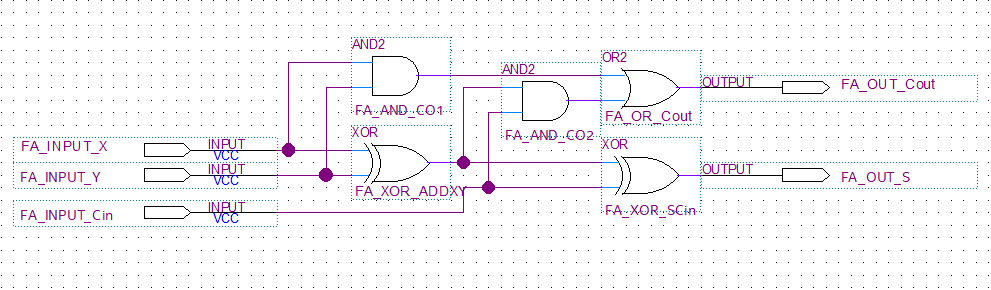
\includegraphics[width=\textwidth]{diagrams/full-adder-logic.PNG}
            \caption{Logic Diagram of Full Adder}
        \end{figure}

        \begin{figure}[!htb]
            \centering
            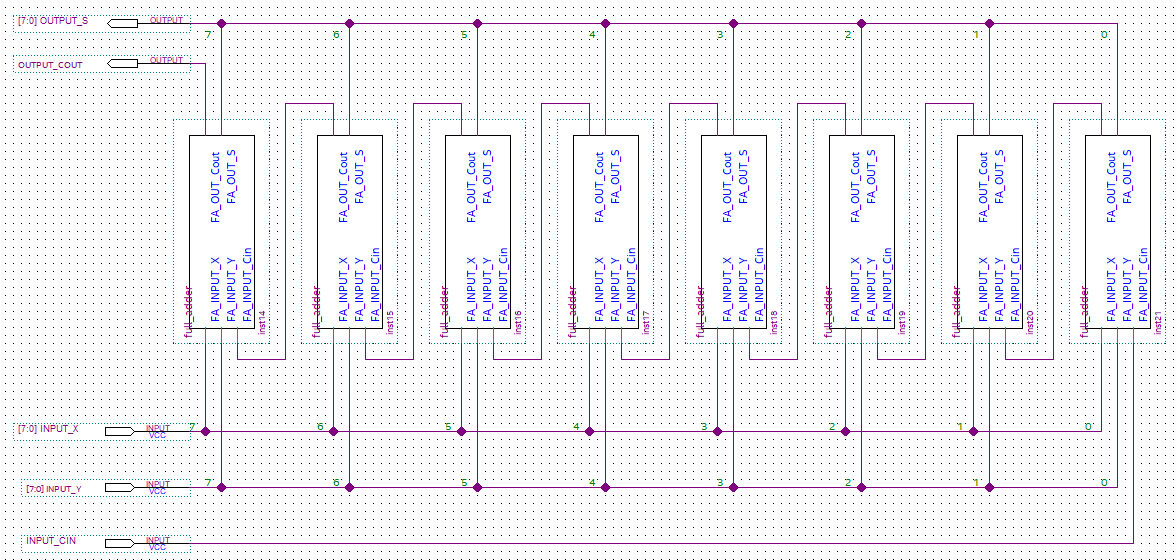
\includegraphics[width=\textwidth]{diagrams/rca-8b-logic.PNG}
            \caption{Logic Diagram of 8bit Ripple Carry Adder}
        \end{figure}

    \chapter{Simulation}
        \section{Source Code}
            \lstinputlisting[caption=Full Adder]{ripple-carry-adder/full_adder_1b.v}
            \lstinputlisting[caption=Full Adder]{ripple-carry-adder/rca_8b_top.v}
        \section{Testbench}
            \lstinputlisting[caption=Full Adder]{ripple-carry-adder/rca_8b_tb.v}

        \section{Simulation Result}
            \begin{figure}[!htb]
                \centering
                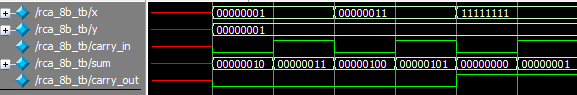
\includegraphics[width=\textwidth]{diagrams/rca-8b-waveform-part1.PNG}
        
                \caption{Waveform: 8-bit Ripple Carry Adder Part1}
                \label{fig:waveform_rca8bp1}
            \end{figure}

            \begin{figure}[!htb]
                \centering
                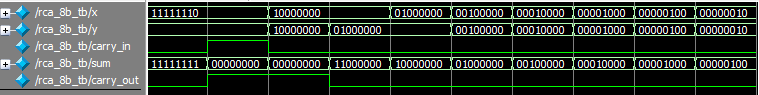
\includegraphics[width=\textwidth]{diagrams/rca-8b-waveform-part2.PNG}
        
                \caption{Waveform: 8-bit Ripple Carry Adder Part2}
                \label{fig:waveform_rca8bp2}
            \end{figure}

            \begin{longtable}[here,width=\textwidth]{|c|c|c|c|c|c|}
                \caption{Result table from Figure~\ref{fig:waveform_rca8bp1} Figure~\ref{fig:waveform_rca8bp2} \label{fig:result_table}}      \\

                \hline
                Case & X                         & Y                         & Cin                & S        & Cout               \\ \hline
                \#01 & \multirow{2}{*}{00000001} & \multirow{8}{*}{00000001} & 0                  & 00000010 & \multirow{4}{*}{0} \\ \cline{1-1} \cline{4-5}
                \#02 &                           &                           & 1                  & 00000011 &                    \\ \cline{1-2} \cline{4-5}
                \#03 & \multirow{2}{*}{00000011} &                           & 0                  & 00000100 &                    \\ \cline{1-1} \cline{4-5}
                \#04 &                           &                           & 1                  & 00000101 &                    \\ \cline{1-2} \cline{4-6} 
                \#05 & \multirow{2}{*}{11111111} &                           & 0                  & 00000000 & \multirow{2}{*}{1} \\ \cline{1-1} \cline{4-5}
                \#06 &                           &                           & 1                  & 00000001 &                    \\ \cline{1-2} \cline{4-6} 
                \#07 & \multirow{2}{*}{11111110} &                           & 0                  & 11111111 & 0                  \\ \cline{1-1} \cline{4-6} 
                \#08 &                           &                           & 1                  & 00000000 & \multirow{2}{*}{1} \\ \cline{1-5}
                \#09 & \multirow{2}{*}{10000000} & 10000000                  & \multirow{8}{*}{0} & 00000000 &                    \\ \cline{1-1} \cline{3-3} \cline{5-6} 
                \#10 &                           & \multirow{2}{*}{01000000} &                    & 11000000 & \multirow{7}{*}{0} \\ \cline{1-2} \cline{5-5}
                \#11 & 01000000                  &                           &                    & 10000000 &                    \\ \cline{1-3} \cline{5-5}
                \#12 & 00100000                  & 00100000                  &                    & 01000000 &                    \\ \cline{1-3} \cline{5-5}
                \#13 & 00010000                  & 00010000                  &                    & 00100000 &                    \\ \cline{1-3} \cline{5-5}
                \#14 & 00001000                  & 00001000                  &                    & 00010000 &                    \\ \cline{1-3} \cline{5-5}
                \#15 & 00000100                  & 00000100                  &                    & 00001000 &                    \\ \cline{1-3} \cline{5-5}
                \#16 & 00000010                  & 00000010                  &                    & 00000100 &                    \\ \hline
            \end{longtable}

    \chapter{Evaluation}
        \paragraph{\normalfont Figure~\ref{fig:waveform_rca8bp1}, Figure~\ref{fig:waveform_rca8bp2}, and Table~\ref{fig:result_table} shows the result of testbench simulation.  }

        \paragraph{\normalfont For the cases \#01 \~ \#08, Carries are successfully passed into next adder, and caused overflow. Also, Every adders can pass its carry to next stage, As if case \#11 \~ \#16.}
    
        \paragraph{\normalfont Therefore, The Ripple Carry Adder is properly designed.}        
    \chapter{Discussions}
        \section{Key Part of This Lab}
            \paragraph{\normalfont In this lab, I've learned about how to draw and symbolize submodules in block diagram. Also, it could be defined as another module, that is able to be utilized in top or any other submodules.}

        \section{Mistakes}
            \begin{figure}[!htb]
                \centering
                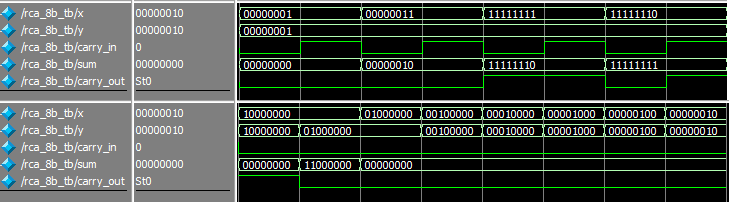
\includegraphics[width=\textwidth]{diagrams/rca-8b-waveform-wrong.png}
                \caption{Wrong waveform due to design error}
            \end{figure}

            \paragraph{\normalfont I initially designed the Full Adder to determine sum as \texttt{ s = x \^{} y } and I got wrong waveforms.}

            \paragraph{\normalfont After I revise the line to \texttt{ s = x \^{} y \^{} cin } then I got the right waveform.}
        \section{Expected Improvements}

            \paragraph{\normalfont From this project, The system will be designed could be larger and complex, requires much more testing cases. }
\end{document}